\documentclass{article}
\usepackage[utf8]{inputenc}
\usepackage{natbib}
\usepackage{graphicx}
\usepackage{amsmath}
\usepackage[nolist]{acronym}% http://ctan.org/pkg/acronym

\begin{document}
\begin{acronym}
\acro{CORLP}    [CORLP]     {Complex Representation-based Link Prediction}
\acro{PCA}    [PCA]     {Principal Component Analysis}
\end{acronym}

%   PAGE:   TITLE
%% Reference of Title Page https://en.wikibooks.org/wiki/LaTeX/Title_Creation
\begin{titlepage}
	\centering
	\begin{figure}[h!]
        \centering
        
\includegraphics[width=0.59\linewidth]{images/logo.png}
    \end{figure}
    
    \vspace{1.5cm}
	{\Large RECOMMENDER SYSTEMS\par}
	\vspace{1cm}
	{\Large MOVIE RECOMMENDATION USING LINK PREDICTION\par}
	\vfill
	{\large 152120141071 - Kerem YALDIZ}
	\vfill

% Bottom of the page
	{\large January 2019\par}
\end{titlepage}

\clearpage
\clearpage

\tableofcontents
\clearpage

\section{Introduction}
Recommender systems are used to estimate rating or preference that a user will assign to an item. Almost every major tech comopany has applied them. Amazon uses it to suggest products, Facebook uses it to recommend people to follow, Netflix uses it to suggest movies and series to watch. Netflix even gave a million dollars to anyone who could increase its system by 10\%.

Recommendation systems have changed the way web sites communicate with their users. Rather than providing content, based on users' search, provides richer experience by indentifying recommendations for every user based on past searches, purchases and votes.

There are majorly six types of recommender systems: collaborative, content-based, demographic based, utility based, Knowledge based and Hybrid recommender system. One of the most popular and promising type is collobrative

There are several types of recommender systems. One of the most promising is the collobrative filtering aproach. It provides recommendations using only user-item interactions. It's divided into two types; item based or user based.~\cite{xie2015link} Collobrative filtering aproaches greatly suffers from data sparcity problem.~\cite{chen2005link}

Collaborative filtering is a great recommendatiton aproach  that uses past user-item interactions for recommendation. By mapping interactions to a bipartite user-item interaction graph, a recommendation problem is converted to a link prediction problem.~\cite{xie2015link}

In this paper, I implemented \ac{CORLP} method using MovieLens dataset.

\section{Methodology}
In this paper, proposed method is based on converting past user-item interactions to graph model. There are two types of nodes, first one is users and the other one is items. In this model, edges between user-item refer to like, edges between user-user and item-item refer to similarity. User-user and item-item link are represented with real numers and user-item link are represented with complex numbers.\cite{xie2015link}

In MovieLens dataset, votes are represented between 1 and 5. Links between users and items refer to like or dislike for that reason they need to be expressed with complex numbers. Vote  (0) is expressed with 0, votes (1,2) are expressed with -j and votes (3,4,5) are expressed with j.\cite{xie2015link} Using this expression, I have created user-item and item-user matrix.

Computing similarity between users and items are essential in \ac{CORLP} method. But when size grows, computing similarity becomes more expensive. For this reason user-item data need to be decompressed. In this paper, I have used \ac{PCA} for decomposition.

When the requirements achieved similarity can be calculated for both users and items. In this paper, I have used pearson correlation to calculate similarity. Using pearson correlation, I have created user-user and item-item similarity matrixes.

Finally, using user-user, user-item, item-user and item-item matrixes, I have created adjacency matrix. Adjacency matrix is 2x2 matrix whose items are
\[
A=
  \begin{bmatrix}
    user-user & user-item \\
    item-user & item-item
  \end{bmatrix}
\]

"Since the power sum of the adjacency matrix measures closeness among nodes, each entry of the top-right component expresses how relevant any item is to a particular user."\cite{xie2015link} After calculating power sum of the adjacency matrix, recommendations can be ranked for each individual user.

\section{Conclusion}
Almost every tech company uses recommendation systems to provide its users a better experience. There are several types of methods to build a recommendation system. One of the most promising one is \ac{CORLP}. In this paper we have implemented \ac{CORLP} with MovieLens dataset.

\subsection{Recommendation Application}
First of all, I have built an application to implement recommendation system. This application is written in Python. I have used pandas, numpy and sklearn modules for implementing recommendation, gpcharts module for drawing charts.

\begin{figure}[h!]
   \centering
   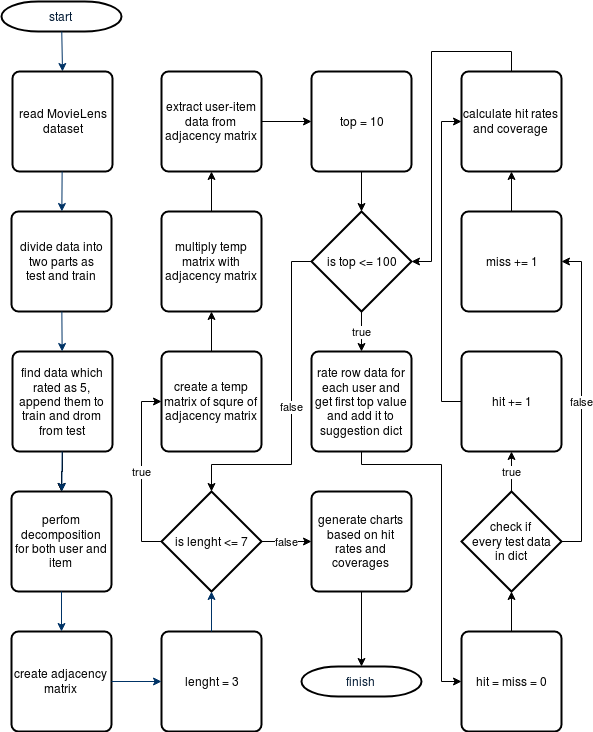
\includegraphics[width=1\linewidth]{images/flowchart.png}
   \caption{Flowchart}
   \label{fig:flowchart}
\end{figure}

As you can see in the figure ~\ref{fig:flowchart} application starts with reading dataset and dividing it into two parts as train and test data. It finds data which is rated as 5 from test data and moves the data from test to train. Perfoms decomposition for both users and items. Replaces NaN with 0, (1,2) with -j and (3,4,5) with j. Performs pearson correlation for both users and items. Creates adjacency matrix using user-user, user-item, item-user and item-item matrixes. Calculates square of adjacency matrix and assigns it to a temporary matrix. Creates a loop for 3, 5 and 7 lengths. Each time multiplies adjacency matrix with temporary matrix and assigns it to a result matrix. Extracts user-item matrix from result matrix. Performs test process if test data is in suggestion list. Performs counting operation based on the result. Calculates hit rates and coverage. Finally generates charts based on the results.

In this application, calculated length values are 3, 5 and 7. Suggestion sizes are 10 to 100 increments 10 each step.

MovieLens dataset contains 943 users, 1682 movies and 100k votes.

Source code for application and report can be found at \url{https://git.keremyaldiz.com/kerem/recommenderSystems} and \url{https://git.keremyaldiz.com/kerem/recommenderSystemsReport}. Both source code is lisenced under GPL-3.0.

\subsection{Results}
As you can see in the figures ~\ref{fig:hits-rate-comparison} and ~\ref{fig:coverage-comparison} are results. For Top-10 and Lenght=3 hits rate is 8.61 and coverage is 10.12. For Top-100 and Lenght=3 hits rate is 44.92 and coverage is 52.17.

\begin{figure}[h!]
   \centering
   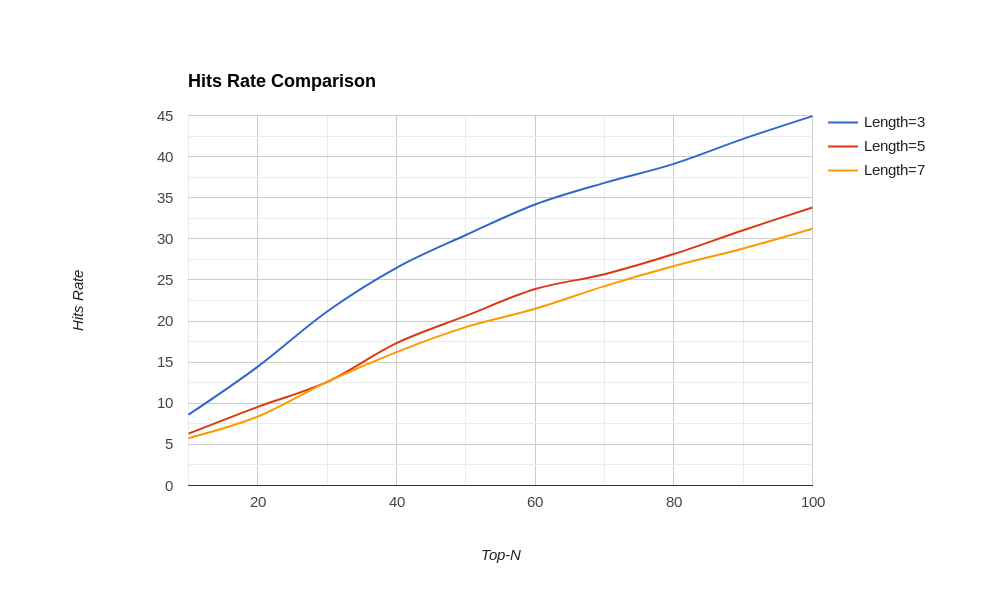
\includegraphics[width=1\linewidth]{images/hits-rate-comparison.png}
   \caption{Hits Rate Comparison}
   \label{fig:hits-rate-comparison}
\end{figure}

\begin{figure}[h!]
   \centering
   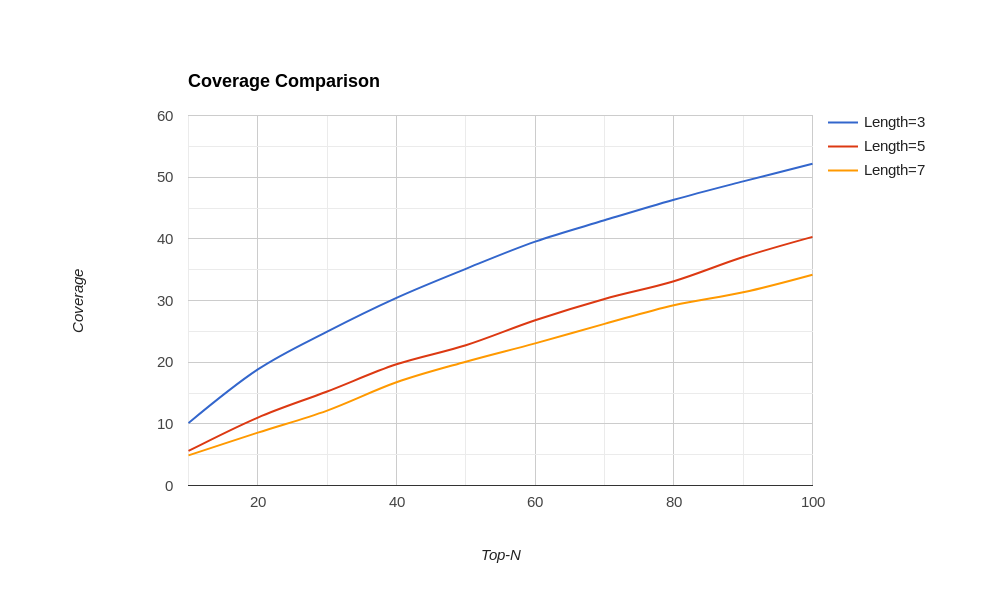
\includegraphics[width=1\linewidth]{images/coverage-comparison.png}
   \caption{Coverage Comparison}
   \label{fig:coverage-comparison}
\end{figure}

This application is executed on a computer with Intel(R) Atom(TM) CPU  C2750  @ 2.40GHz 8 cores 1 thread per CPU. Memory with 32GB RAM and SSD disk. Operating system Ubuntu 18.04.1 LTS.
\[
time=
  \begin{bmatrix}
    real & 0m53.059s \\
    user & 4m30.980s \\
    sys & 0m9.310s
  \end{bmatrix}
\]

\clearpage
\bibliographystyle{plain}
\bibliography{references}
\end{document}